\documentclass[a4paper,11pt]{article}

\usepackage[margin=1.5cm]{geometry}
\usepackage{graphicx}
\usepackage{titlesec}
\usepackage{parskip}
\usepackage{fancyhdr}
\usepackage{hyperref}

\pagestyle{empty}

% Section formatting
\titleformat{\section}{\bfseries\normalsize}{}{0em}{}
\titleformat{\subsection}{\bfseries\small}{}{0em}{}

\begin{document}

\textbf{Group 13} \hfill \textbf{\today}

\vspace{0.5em}
Niklas Oswald\\
Abdulrahman Bingharamah

\vspace{1em}
\begin{center}
    \textbf{\large Passau Flood Explorer}
\end{center}

\section*{Goal}
Passau lies at the confluence of Danube, Inn, and Ilz and has a long flood history (e.g. 1954, 2013). The goal of our project is to simulate and visualize the rising water levels of these rivers and use asymmetric cross-device collaboration to analyze and understand flood development in the city of Passau. This should enable the users to explore and analyze historical flood events, identify potentially affected and critical areas and buildings and explore protection scenarios for expected future floods.

Our application will be designed to allow two users to simultaneously collaborate on achieving these goals. A desktop user (analyst), who has an overview of the whole city, will be responsible for picking the scenario (water levels, warning level, historical event), filtering and annotating specific areas or buildings and guiding the VR user. The VR user (explorer) will use embodied, spatial exploration at human scale to mark and annotate critical areas, which are not apparent in the overview perspective of the Desktop user, and use this information to place protection barriers in order to explore potential protection scenarios and their effectiveness.

The ''Passau Flood Explorer'' will enable the following analysis tasks: Which buildings are affected at a given water level? How deep would the water be at a specific place? Which routes are blocked first? Where could a barrier protect the most buildings?

\section*{Design Considerations / Selected Visualizations}
The application is planned as an asymmetric cross-device collaboration system in which both, the desktop user as well as the VR user, have a individual analytical purpose. 

The 2D desktop environment will be used to set up the simulation, highlight/annotate critical and interesting areas, which may require a more detailed investigation by the VR user, control the scenario during the simulation and analyze potential protection scenarios emerging from the collaborative exploration. \\
Setting up the simulation involves choosing a historical flooding event or creating a custom future flooding scenario and setting the simulation speed. Choosing between different historical events and creating custom scenarios will be supported by a hydrograph displaying the water levels over time. \\
To highlight and annotate certain areas and buildings the city will be presented as a 2D map to the desktop user, who can arbitrarily zoom in and out to focus on specific areas and facilitate annotating/highlighting. Highlighting areas/buildings uses region highlighting with different colors to emphasize critical or interesting areas. Annotations will be presented as point-of-interest (POI) markers. An overview of all currently active highlighted areas and markers will be presented in a visual elements panel, allowing the user to efficiently manage them. Clicking on one of the visual elements in the panel will also shift the user's focus on the map to the respective area.\\
During the simulation, the desktop user will be able to control the simulation speed, pause at certain points in time and add further visual elements.

Using the Pimax Crystal Super or the HTC VIVE Pro 2, the VR user will be fully immersed in the 3D surface-rendered city of Passau in a first-person perspective. The VR user's main purpose will be to investigate certain areas in more detail, which would not be possible in the plain 2D view. This includes identifying whether the water depth actually causes problems at certain areas or buildings and which routes will be blocked by the water as well as exploring potentially useful positions for protection barriers.\\
To this end, the VR user will be able to freely walk or fly through the city at human scale and communicate their findings to the desktop user. Furthermore, it will be possible to quickly teleport to a different part of the city using World-in-Miniature (WIM) navigation. Using the VR controllers, the user can further highlight and annotate certain areas and buildings and also place protection barriers.\\
This efficient embodied exploration should convey a sense of spatial presence, which is supposed to significantly improve the user's ability of identifying critical areas and creating and analyzing potential protection scenarios. 

As an asymmetric collaboration application, each of the users' actions will also be displayed in the respective other environment. This means that areas highlighted by the desktop user will appear as a 3D color mapping in the virtual environment and vice versa. The same applies to annotations made by either of the users while the placement of protection barriers made by the VR user will also be accordingly visualized in the desktop environment.\\
Moreover, the VR user's position and orientation in the city will be indicated as a small cone on the desktop user's map to make it easier to guide the VR user.

We will use LoD2 (Level of Detail 2) 3D building data from OpenData\footnote{\url{https://geodaten.bayern.de/opengeodata/OpenDataDetail.html?pn=lod2}} to model the city of Passau in the virtual environment. This dataset is provided in CityGML format and may be supported by further data coming from OpenStreetMap\footnote{\url{https://www.openstreetmap.de/}} if required. To simulate floods, water level data will be retrieved from the Bavarian Hydrological Service\footnote{\url{https://www.gkd.bayern.de/}} in CSV format and complemented by GeoPackage data from the Bavarian Environment Agency\footnote{\url{https://www.lfu.bayern.de/umweltdaten/geodatendienste/pretty\_downloaddienst.htm?dld=hochwasserereignisse\_g1\_g2.xml}}.

\textbf{Mockups}

\begin{center}
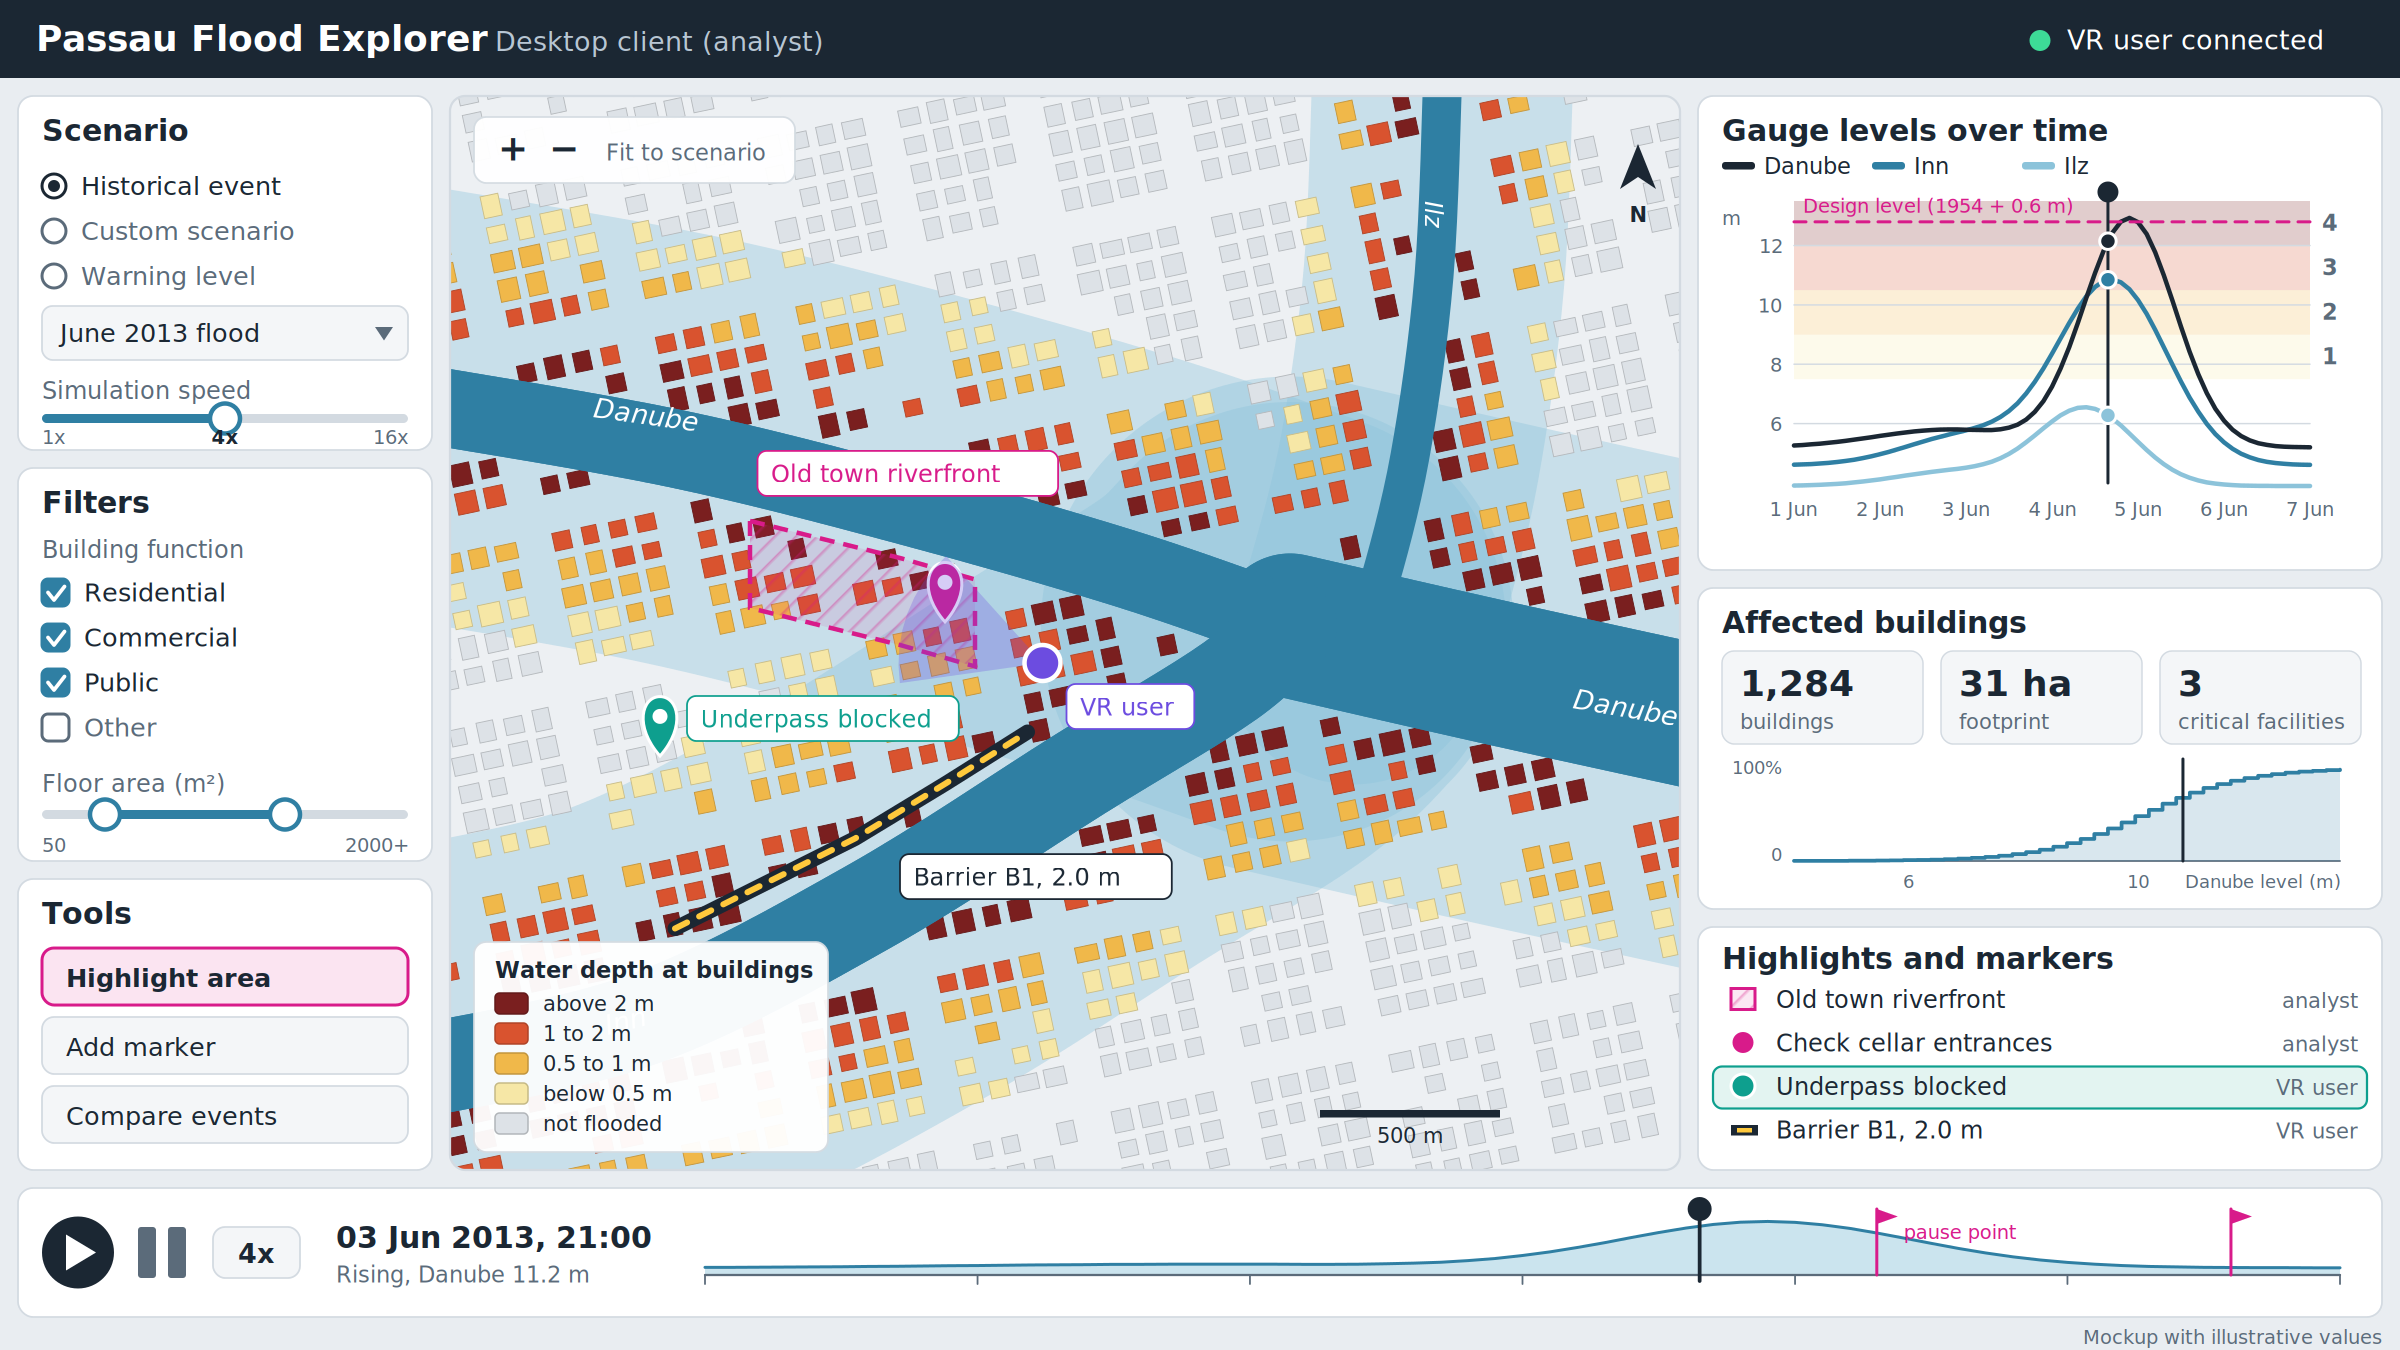
\includegraphics[
    width=\linewidth,
    height=0.72\textheight,
    keepaspectratio
]{images/mockup_desktop.png}
\end{center}
\footnotesize Figure 1: Desktop environment mockup

\begin{center}
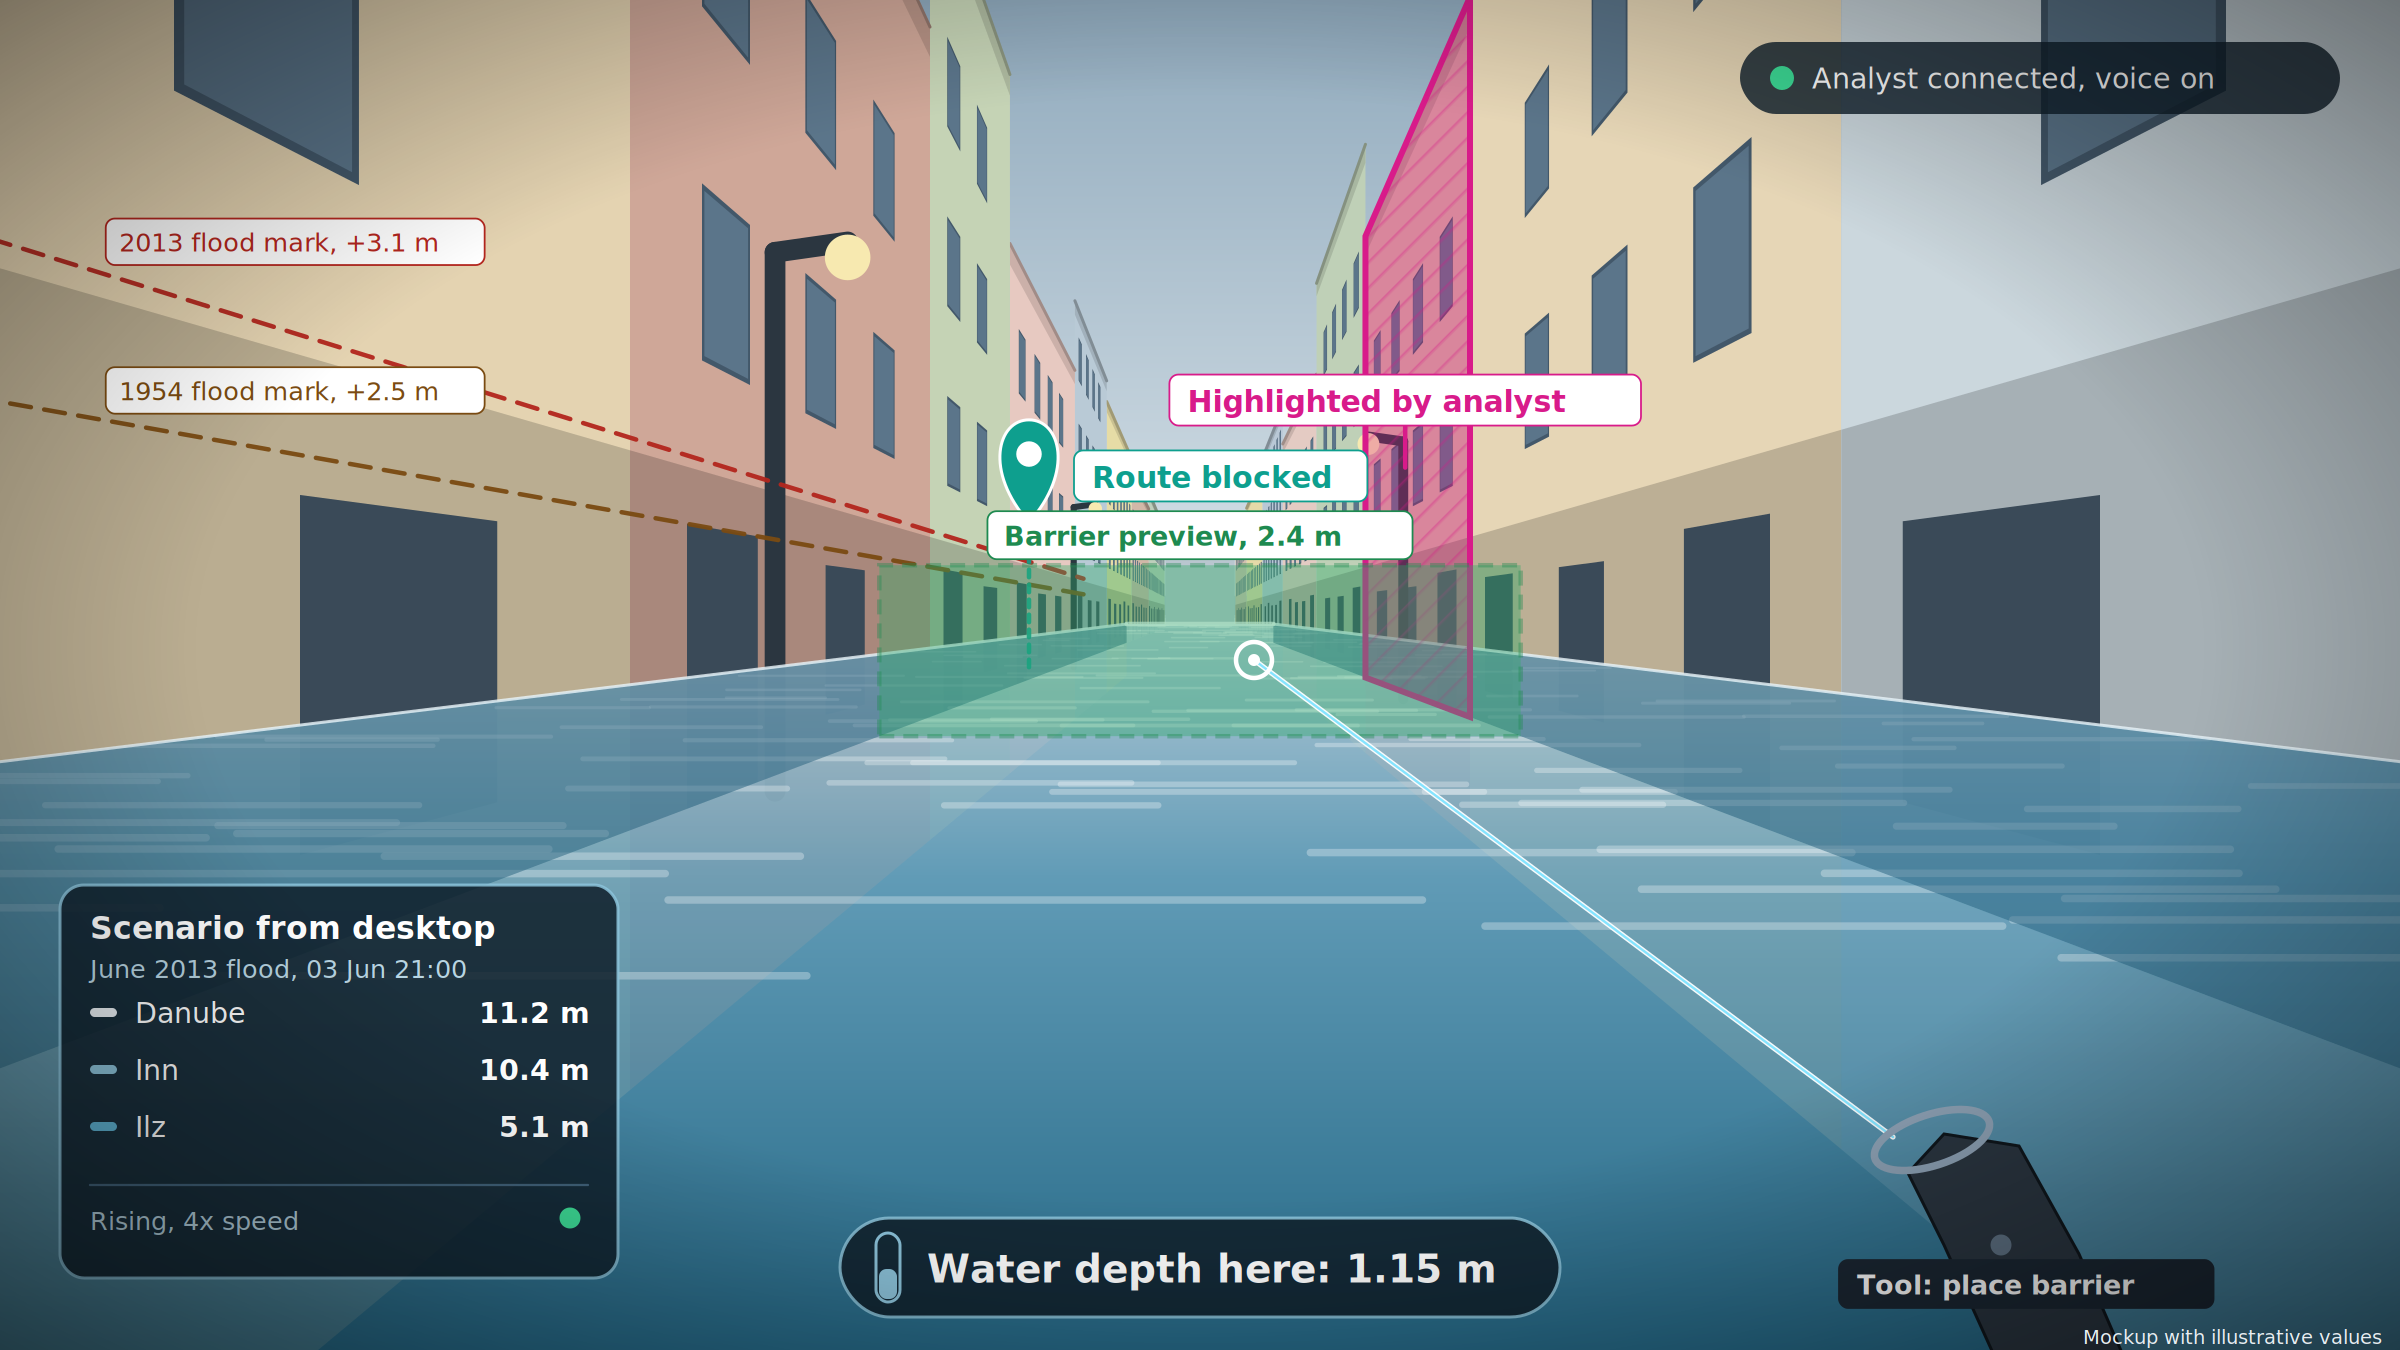
\includegraphics[
    width=\linewidth,
    height=0.72\textheight,
    keepaspectratio
]{images/mockup_vr_street.png}
\end{center}
\footnotesize Figure 2: Virtual environment mockup


\vspace{1.5em}

\end{document}
